%\SweaveUTF8
\documentclass[aspectratio=169]{beamer}

\usetheme{default}
% Slide setup, colour independent

\usepackage{amsmath,amssymb,amsthm}
\usepackage[utf8]{inputenc}
\usepackage{colortbl}
\usepackage{bm}
\usepackage{xcolor}
\usepackage{dsfont}
\usepackage{setspace}
%\usepackage{subfigure}
% To use \ding{234} and the like
\usepackage{pifont}
% To cross reference between slide files
\usepackage{zref-xr,zref-user}
% Use something like
% \zexternaldocument{fileI}
% in the tex files. And cite using \zref instead of \ref
\usepackage{booktabs}
\usepackage{marvosym}
\usepackage{cancel}
%\usepackage{transparent}

% Fields and the like
\def\IC{\mathbb{C}}
\def\IE{\mathbb{E}}
\def\IF{\mathbb{F}}
\def\II{\mathbb{I}}
\def\IJ{\mathbb{J}}
\def\IK{\mathbb{K}}
\def\IM{\mathbb{M}}
\def\IN{\mathbb{N}}
\def\IP{\mathbb{P}}
\def\IR{\mathbb{R}}
\def\IZ{\mathbb{Z}}
\def\11{\mathds{1}}


% Bold lowercase
\def\ba{\bm{a}}
\def\bb{\bm{b}}
\def\bc{\bm{c}}
\def\bd{\bm{d}}
\def\be{\bm{e}}
\def\bf{\bm{f}}
\def\bh{\bm{h}}
\def\bi{\bm{i}}
\def\bj{\bm{j}}
\def\bk{\bm{k}}
\def\bn{\bm{n}}
\def\bp{\bm{p}}
\def\br{\bm{r}}
\def\bs{\bm{s}}
\def\bu{\bm{u}}
\def\bv{\bm{v}}
\def\bw{\bm{w}}
\def\bx{\bm{x}}
\def\by{\bm{y}}
\def\bz{\bm{z}}

% Bold capitals
\def\bB{\bm{B}}
\def\bD{\bm{D}}
\def\bE{\bm{E}}
\def\bF{\bm{F}}
\def\bG{\bm{G}}
\def\bI{\bm{I}}
\def\bL{\bm{L}}
\def\bN{\bm{N}}
\def\bP{\bm{P}}
\def\bR{\bm{R}}
\def\bS{\bm{S}}
\def\bT{\bm{T}}
\def\bX{\bm{X}}

% Bold numbers
\def\b0{\bm{0}}

% Bold greek
\bmdefine{\bmu}{\bm{\mu}}
\def\bphi{\bm{\phi}}
\def\bvarphi{\bm{\varphi}}
\def\bPi{\bm{\Pi}}
\def\bGamma{\bm{\Gamma}}

% Bold red sentence
\def\boldred#1{{\color{red}\textbf{#1}}}
\def\defword#1{{\color{orange}\textbf{#1}}}

% Caligraphic letters
\def\A{\mathcal{A}}
\def\B{\mathcal{B}}
\def\C{\mathcal{C}}
\def\D{\mathcal{D}}
\def\E{\mathcal{E}}
\def\F{\mathcal{F}}
\def\G{\mathcal{G}}
\def\H{\mathcal{H}}
\def\I{\mathcal{I}}
\def\L{\mathcal{L}}
\def\M{\mathcal{M}}
\def\N{\mathcal{N}}
\def\P{\mathcal{P}}
\def\R{\mathcal{R}}
\def\S{\mathcal{S}}
\def\T{\mathcal{T}}
\def\U{\mathcal{U}}
\def\V{\mathcal{V}}

% Adding space for prime (') where needed
\def\pprime{\,'}
% Adding space for star (\star) where needed
\def\pstar{{\,\star}}

% tt font for code
\def\code#1{{\tt #1}}

% i.e., e.g.
\def\eg{\emph{e.g.}}
\def\ie{\emph{i.e.}}


% Operators and special symbols
\def\nbOne{{\mathchoice {\rm 1\mskip-4mu l} {\rm 1\mskip-4mu l}
{\rm 1\mskip-4.5mu l} {\rm 1\mskip-5mu l}}}
\def\cov{\ensuremath{\mathsf{cov}}}
\def\Var{\ensuremath{\mathsf{Var}\ }}
\def\Im{\textrm{Im}\;}
\def\Re{\textrm{Re}\;}
\def\det{\ensuremath{\mathsf{det}}}
\def\diag{\ensuremath{\mathsf{diag}}}
\def\nullspace{\ensuremath{\mathsf{null}}}
\def\nullity{\ensuremath{\mathsf{nullity}}}
\def\rank{\ensuremath{\mathsf{rank}}}
\def\range{\ensuremath{\mathsf{range}}}
\def\sgn{\ensuremath{\mathsf{sgn}}}
\def\Span{\ensuremath{\mathsf{span}}}
\def\tr{\ensuremath{\mathsf{tr}}}
\def\imply{$\Rightarrow$}
\def\restrictTo#1#2{\left.#1\right|_{#2}}
\newcommand{\parallelsum}{\mathbin{\!/\mkern-5mu/\!}}
\def\dsum{\mathop{\displaystyle \sum }}%
\def\dind#1#2{_{\substack{#1\\ #2}}}

\DeclareMathOperator{\GL}{GL}
\DeclareMathOperator{\Rel}{Re}
\def\Nt#1{\left|\!\left|\!\left|#1\right|\!\right|\!\right|}
\newcommand{\tripbar}{|\! |\! |}



% The beamer bullet (in base colour)
\def\bbullet{\leavevmode\usebeamertemplate{itemize item}\ }

% Theorems and the like
\newtheorem{proposition}[theorem]{Proposition}
\newtheorem{property}[theorem]{Property}
\newtheorem{importantproperty}[theorem]{Property}
\newtheorem{importanttheorem}[theorem]{Theorem}
%\newtheorem{lemma}[theorem]{Lemma}
%\newtheorem{corollary}[theorem]{Corollary}
\newtheorem{remark}[theorem]{Remark}
\setbeamertemplate{theorems}[numbered]
%\setbeamertemplate{theorems}[ams style]

%
%\usecolortheme{orchid}
%\usecolortheme{orchid}

\def\red{\color[rgb]{1,0,0}}
\def\blue{\color[rgb]{0,0,1}}
\def\green{\color[rgb]{0,1,0}}


% Get rid of navigation stuff
\setbeamertemplate{navigation symbols}{}

% Set footline/header line
\setbeamertemplate{footline}
{%
\quad p. \insertpagenumber \quad--\quad \insertsection\vskip2pt
}
% \setbeamertemplate{headline}
% {%
% \quad\insertsection\hfill p. \insertpagenumber\quad\mbox{}\vskip2pt
% }


\makeatletter
\newlength\beamerleftmargin
\setlength\beamerleftmargin{\Gm@lmargin}
\makeatother

% Colours for special pages
\def\extraContent{yellow!20}


%%%%%%%%%%%%%%%%%
\usepackage{tikz}
\usetikzlibrary{shapes,arrows}
\usetikzlibrary{positioning}
\usetikzlibrary{shapes.symbols,shapes.callouts,patterns}
\usetikzlibrary{calc,fit}
\usetikzlibrary{backgrounds}
\usetikzlibrary{decorations.pathmorphing,fit,petri}
\usetikzlibrary{automata}
\usetikzlibrary{fadings}
\usetikzlibrary{patterns,hobby}
\usetikzlibrary{backgrounds,fit,petri}
\usetikzlibrary{tikzmark}

\usepackage{pgfplots}
\pgfplotsset{compat=1.6}
\pgfplotsset{ticks=none}

\usetikzlibrary{decorations.markings}
\usetikzlibrary{arrows.meta}
\tikzset{>=stealth}

% For tikz
\tikzstyle{cloud} = [draw, ellipse,fill=red!20, node distance=0.87cm,
minimum height=2em]
\tikzstyle{line} = [draw, -latex']


%%% For max frame images
\newenvironment{changemargin}[2]{%
\begin{list}{}{%
\setlength{\topsep}{0pt}%
\setlength{\leftmargin}{#1}%
\setlength{\rightmargin}{#2}%
\setlength{\listparindent}{\parindent}%
\setlength{\itemindent}{\parindent}%
\setlength{\parsep}{\parskip}%
}%
\item[]}{\end{list}}


% Make one image take up the entire slide content area in beamer,.:
% centered/centred full-screen image, with title:
% This uses the whole screen except for the 1cm border around it
% all. 128x96mm
\newcommand{\titledFrameImage}[2]{
\begin{frame}{#1}
%\begin{changemargin}{-1cm}{-1cm}
\begin{center}
\includegraphics[width=108mm,height=\textheight,keepaspectratio]{#2}
\end{center}
%\end{changemargin}
\end{frame}
}

% Make one image take up the entire slide content area in beamer.:
% centered/centred full-screen image, no title:
% This uses the whole screen except for the 1cm border around it
% all. 128x96mm
\newcommand{\plainFrameImage}[1]{
\begin{frame}[plain]
%\begin{changemargin}{-1cm}{-1cm}
\begin{center}
\includegraphics[width=108mm,height=76mm,keepaspectratio]{#1}
\end{center}
%\end{changemargin}
\end{frame}
}

% Make one image take up the entire slide area, including borders, in beamer.:
% centered/centred full-screen image, no title:
% This uses the entire whole screen
\newcommand{\maxFrameImage}[1]{
\begin{frame}[plain]
\begin{changemargin}{-1cm}{-1cm}
\begin{center}
\includegraphics[width=\paperwidth,height=\paperheight,keepaspectratio]
{#1}
\end{center}
\end{changemargin}
\end{frame}
}

% This uses the entire whole screen (to include in frame)
\newcommand{\maxFrameImageNoFrame}[1]{
\begin{changemargin}{-1cm}{-1cm}
\begin{center}
\includegraphics[width=\paperwidth,height=0.99\paperheight,keepaspectratio]
{#1}
\end{center}
\end{changemargin}
}

% Make one image take up the entire slide area, including borders, in beamer.:
% centered/centred full-screen image, no title:
% This uses the entire whole screen
\newcommand{\maxFrameImageColor}[2]{
\begin{frame}[plain]
\setbeamercolor{normal text}{bg=#2!20}
\begin{changemargin}{-1cm}{-1cm}
\begin{center}
\includegraphics[width=\paperwidth,height=\paperheight,keepaspectratio]
{#1}
\end{center}
\end{changemargin}
\end{frame}
}


\usepackage{tikz}
\usetikzlibrary{patterns,hobby}
\usepackage{pgfplots}
\pgfplotsset{compat=1.6}
\pgfplotsset{ticks=none}

\usetikzlibrary{backgrounds}
\usetikzlibrary{decorations.markings}
\usetikzlibrary{arrows.meta}
\tikzset{>=stealth}

\tikzset{
  clockwise arrows/.style={
    postaction={
      decorate,
      decoration={
        markings,
        mark=between positions 0.1 and 0.9 step 40pt with {\arrow{>}},
   }}}}


% Beginning of a section
\newcommand{\newSectionSlide}[1]{
\begin{frame}[noframenumbering,plain]
  \begin{tikzpicture}[remember picture,overlay]
    \node[above right,inner sep=0pt,opacity=0.2] at (current page.south west)
    {
        \includegraphics[height=\paperheight,width=\paperwidth]{#1}
    };
  \end{tikzpicture}
  \setbeamercolor{section in toc}{fg=subsub_header_section}
  \setbeamerfont{section in toc}{size=\Large,series=\bfseries}
  \setbeamertemplate{section in toc shaded}[default][60]
  %\setbeamercolor{background canvas}{bg=section_colour}
  \tableofcontents[
    currentsection,
    sectionstyle=show/shaded,
    subsectionstyle=show/hide/hide,
    subsubsectionstyle=hide/hide/hide]
\end{frame}
\addtocounter{page}{-1}
}

% Beginning of a subsection
\newcommand{\newSubSectionSlide}[1]{
\begin{frame}[noframenumbering,plain]
  \begin{tikzpicture}[remember picture,overlay]
    \node[above right,inner sep=0pt,opacity=0.2] at (current page.south west)
    {
        \includegraphics[height=\paperheight,width=\paperwidth]{#1}
    };
  \end{tikzpicture}
  \setbeamercolor{section in toc}{fg=subsub_header_section}
  \setbeamerfont{section in toc}{size=\Large,series=\bfseries}
  \setbeamertemplate{section in toc shaded}[default][60]
  %\setbeamercolor{background canvas}{bg=section_colour}
  \tableofcontents[
    currentsection,
    sectionstyle=show/hide,
    subsectionstyle=show/shaded/hide,
    subsubsectionstyle=hide/hide/hide]
\end{frame}
\addtocounter{page}{-1}
}



   %%%%%%%%%%%
% To have links to parts in the outline
\makeatletter
\AtBeginPart{%
  \addtocontents{toc}{\protect\beamer@partintoc{\the\c@part}{\beamer@partnameshort}{\the\c@page}}%
}
%% number, shortname, page.
\providecommand\beamer@partintoc[3]{%
  \ifnum\c@tocdepth=-1\relax
    % requesting onlyparts.
    \makebox[6em]{Part #1:} \textcolor{green!30!blue}{\hyperlink{#2}{#2}}
    \par
  \fi
}
\define@key{beamertoc}{onlyparts}[]{%
  \c@tocdepth=-1\relax
}
\makeatother%

\newcommand{\nameofthepart}{}
\newcommand{\nupart}[1]%
    {   \part{#1}%
        \renewcommand{\nameofthepart}{#1}%
        {
          \setbeamercolor{background canvas}{bg=orange!50}
          \begin{frame}{#1}%\partpage 
          \hypertarget{\nameofthepart}{}\tableofcontents%
          \end{frame}
        }
    }


% The title page with figure
\newcommand{\titlepagewithfigure}[1]{%
\begin{frame}[noframenumbering,plain]
  \begin{tikzpicture}[remember picture,overlay]
    \node[above right,inner sep=0pt,opacity=0.2] at (current page.south west)
    {
        \includegraphics[height=\paperheight,width=\paperwidth]{#1}
    };
    \node[anchor=north east,
    inner sep=5pt,
    opacity=0.9] at (current page.north east)
    {
        
\includegraphics[width=0.2\textwidth]{FIGS/UM-logo-horizontal-CMYK.png}
    };
    \node[anchor=south, 
    align=justify, 
    text=black, 
    text width=1.1\textwidth,
    font=\footnotesize]  (land_acknowledgement)
    at (current page.south) 
    {The University of Manitoba campuses are located on original lands of Anishinaabeg, Ininew, Anisininew, Dakota and Dene peoples, and on the National Homeland of the Red River Métis.\\
    We respect the Treaties that were made on these territories, we acknowledge the harms and mistakes of the past, and we dedicate ourselves to move forward in partnership with Indigenous communities in a spirit of Reconciliation and collaboration.};  
    \node[align=center, anchor=south,
    above=0.5cm of land_acknowledgement,
    text=black,
    font=\bfseries] {Fall 2024};
\end{tikzpicture}
  \setbeamercolor{title}{fg=subsub_header_section}
  \setbeamercolor{author}{fg=subsub_header_section} 
  \setbeamerfont{title}{size=\Large,series=\bfseries}
  \setbeamerfont{author}{size=\Large,series=\bfseries}
  \setbeamerfont{date}{series=\bfseries}
	\titlepage
\end{frame}
\addtocounter{page}{-1}
}


% The outline page, with figure
\newcommand{\outlinepage}[1]{%
\begin{frame}[noframenumbering,plain]
  \begin{tikzpicture}[remember picture,overlay]
    \node[above right,inner sep=0pt,opacity=0.2] at (current page.south west)
    {
        \includegraphics[height=\paperheight,width=\paperwidth]{#1}
    };
  \end{tikzpicture}
  \setbeamercolor{section in toc}{fg=subsub_header_section}
  \setbeamerfont{section in toc}{size=\Large,series=\bfseries}
  \frametitle{\textcolor{blue}{\LARGE\bfseries Outline}}
  \tableofcontents[hideallsubsections]
\end{frame}
\addtocounter{page}{-1}
}




\usecolortheme{orchid}
%% Listings
\usepackage{listings}
\definecolor{mygreen}{rgb}{0,0.6,0}
\definecolor{mygray}{rgb}{0.5,0.5,0.5}
\definecolor{mymauve}{rgb}{0.58,0,0.82}
\definecolor{mygold}{rgb}{1,0.843,0}
\definecolor{myblue}{rgb}{0.537,0.812,0.941}

\definecolor{mygold2}{RGB}{120,105,22}
\definecolor{mygrey2}{RGB}{50,50,50}

\definecolor{lgreen}{rgb}{0.6,0.9,.6}
\definecolor{lred}{rgb}{1,0.5,.5}

\lstloadlanguages{R}
\lstset{ %
  language=R,
  backgroundcolor=\color{black!05},   % choose the background color
  basicstyle=\footnotesize\ttfamily,        % size of fonts used for the code
  breaklines=true,                 % automatic line breaking only at whitespace
  captionpos=b,                    % sets the caption-position to bottom
  commentstyle=\color{mygreen},    % comment style
  escapeinside={\%*}{*)},          % if you want to add LaTeX within your code
  keywordstyle=\color{red},       % keyword style
  stringstyle=\color{mygold},     % string literal style
  keepspaces=true,
  columns=fullflexible,
  tabsize=4,
}
% Could also do (in lstset)
% basicstyle==\fontfamily{pcr}\footnotesize
\lstdefinelanguage{Renhanced}%
  {keywords={abbreviate,abline,abs,acos,acosh,action,add1,add,%
      aggregate,alias,Alias,alist,all,anova,any,aov,aperm,append,apply,%
      approx,approxfun,apropos,Arg,args,array,arrows,as,asin,asinh,%
      atan,atan2,atanh,attach,attr,attributes,autoload,autoloader,ave,%
      axis,backsolve,barplot,basename,besselI,besselJ,besselK,besselY,%
      beta,binomial,body,box,boxplot,break,browser,bug,builtins,bxp,by,%
      c,C,call,Call,case,cat,category,cbind,ceiling,character,char,%
      charmatch,check,chol,chol2inv,choose,chull,class,close,cm,codes,%
      coef,coefficients,co,col,colnames,colors,colours,commandArgs,%
      comment,complete,complex,conflicts,Conj,contents,contour,%
      contrasts,contr,control,helmert,contrib,convolve,cooks,coords,%
      distance,coplot,cor,cos,cosh,count,fields,cov,covratio,wt,CRAN,%
      create,crossprod,cummax,cummin,cumprod,cumsum,curve,cut,cycle,D,%
      data,dataentry,date,dbeta,dbinom,dcauchy,dchisq,de,debug,%
      debugger,Defunct,default,delay,delete,deltat,demo,de,density,%
      deparse,dependencies,Deprecated,deriv,description,detach,%
      dev2bitmap,dev,cur,deviance,off,prev,,dexp,df,dfbetas,dffits,%
      dgamma,dgeom,dget,dhyper,diag,diff,digamma,dim,dimnames,dir,%
      dirname,dlnorm,dlogis,dnbinom,dnchisq,dnorm,do,dotplot,double,%
      download,dpois,dput,drop,drop1,dsignrank,dt,dummy,dump,dunif,%
      duplicated,dweibull,dwilcox,dyn,edit,eff,effects,eigen,else,%
      emacs,end,environment,env,erase,eval,equal,evalq,example,exists,%
      exit,exp,expand,expression,External,extract,extractAIC,factor,%
      fail,family,fft,file,filled,find,fitted,fivenum,fix,floor,for,%
      For,formals,format,formatC,formula,Fortran,forwardsolve,frame,%
      frequency,ftable,ftable2table,function,gamma,Gamma,gammaCody,%
      gaussian,gc,gcinfo,gctorture,get,getenv,geterrmessage,getOption,%
      getwd,gl,glm,globalenv,gnome,GNOME,graphics,gray,grep,grey,grid,%
      gsub,hasTsp,hat,heat,help,hist,home,hsv,httpclient,I,identify,if,%
      ifelse,Im,image,\%in\%,index,influence,measures,inherits,install,%
      installed,integer,interaction,interactive,Internal,intersect,%
      inverse,invisible,IQR,is,jitter,kappa,kronecker,labels,lapply,%
      layout,lbeta,lchoose,lcm,legend,length,levels,lgamma,library,%
      licence,license,lines,list,lm,load,local,locator,log,log10,log1p,%
      log2,logical,loglin,lower,lowess,ls,lsfit,lsf,ls,machine,Machine,%
      mad,mahalanobis,make,link,margin,match,Math,matlines,mat,matplot,%
      matpoints,matrix,max,mean,median,memory,menu,merge,methods,min,%
      missing,Mod,mode,model,response,mosaicplot,mtext,mvfft,na,nan,%
      names,omit,nargs,nchar,ncol,NCOL,new,next,NextMethod,nextn,%
      nlevels,nlm,noquote,NotYetImplemented,NotYetUsed,nrow,NROW,null,%
      numeric,\%o\%,objects,offset,old,on,Ops,optim,optimise,optimize,%
      options,or,order,ordered,outer,package,packages,page,pairlist,%
      pairs,palette,panel,par,parent,parse,paste,path,pbeta,pbinom,%
      pcauchy,pchisq,pentagamma,persp,pexp,pf,pgamma,pgeom,phyper,pico,%
      pictex,piechart,Platform,plnorm,plogis,plot,pmatch,pmax,pmin,%
      pnbinom,pnchisq,pnorm,points,poisson,poly,polygon,polyroot,pos,%
      postscript,power,ppoints,ppois,predict,preplot,pretty,Primitive,%
      print,prmatrix,proc,prod,profile,proj,prompt,prop,provide,%
      psignrank,ps,pt,ptukey,punif,pweibull,pwilcox,q,qbeta,qbinom,%
      qcauchy,qchisq,qexp,qf,qgamma,qgeom,qhyper,qlnorm,qlogis,qnbinom,%
      qnchisq,qnorm,qpois,qqline,qqnorm,qqplot,qr,Q,qty,qy,qsignrank,%
      qt,qtukey,quantile,quasi,quit,qunif,quote,qweibull,qwilcox,%
      rainbow,range,rank,rbeta,rbind,rbinom,rcauchy,rchisq,Re,read,csv,%
      csv2,fwf,readline,socket,real,Recall,rect,reformulate,regexpr,%
      relevel,remove,rep,repeat,replace,replications,report,require,%
      resid,residuals,restart,return,rev,rexp,rf,rgamma,rgb,rgeom,R,%
      rhyper,rle,rlnorm,rlogis,rm,rnbinom,RNGkind,rnorm,round,row,%
      rownames,rowsum,rpois,rsignrank,rstandard,rstudent,rt,rug,runif,%
      rweibull,rwilcox,sample,sapply,save,scale,scan,scan,screen,sd,se,%
      search,searchpaths,segments,seq,sequence,setdiff,setequal,set,%
      setwd,show,sign,signif,sin,single,sinh,sink,solve,sort,source,%
      spline,splinefun,split,sqrt,stars,start,stat,stem,step,stop,%
      storage,strstrheight,stripplot,strsplit,structure,strwidth,sub,%
      subset,substitute,substr,substring,sum,summary,sunflowerplot,svd,%
      sweep,switch,symbol,symbols,symnum,sys,status,system,t,table,%
      tabulate,tan,tanh,tapply,tempfile,terms,terrain,tetragamma,text,%
      time,title,topo,trace,traceback,transform,tri,trigamma,trunc,try,%
      ts,tsp,typeof,unclass,undebug,undoc,union,unique,uniroot,unix,%
      unlink,unlist,unname,untrace,update,upper,url,UseMethod,var,%
      variable,vector,Version,vi,warning,warnings,weighted,weights,%
      which,while,window,write,\%x\%,x11,X11,xedit,xemacs,xinch,xor,%
      xpdrows,xy,xyinch,yinch,zapsmall,zip},%
   otherkeywords={!,!=,~,$,*,\%,\&,\%/\%,\%*\%,\%\%,<-,<<-,_,/},%
   alsoother={._$},%
   sensitive,%
   morecomment=[l]\#,%
   morestring=[d]",%
   morestring=[d]'% 2001 Robert Denham
  }%

%%%%%%% 
%% Definitions in yellow boxes
\usepackage{etoolbox}
\setbeamercolor{block title}{use=structure,fg=structure.fg,bg=structure.fg!40!bg}
\setbeamercolor{block body}{parent=normal text,use=block title,bg=block title.bg!20!bg}

\BeforeBeginEnvironment{definition}{%
	\setbeamercolor{block title}{fg=black,bg=yellow!20!white}
	\setbeamercolor{block body}{fg=black, bg=yellow!05!white}
}
\AfterEndEnvironment{definition}{
	\setbeamercolor{block title}{use=structure,fg=structure.fg,bg=structure.fg!20!bg}
	\setbeamercolor{block body}{parent=normal text,use=block title,bg=block title.bg!50!bg, fg=black}
}
\BeforeBeginEnvironment{importanttheorem}{%
	\setbeamercolor{block title}{fg=black,bg=red!20!white}
	\setbeamercolor{block body}{fg=black, bg=red!05!white}
}
\AfterEndEnvironment{importanttheorem}{
	\setbeamercolor{block title}{use=structure,fg=structure.fg,bg=structure.fg!20!bg}
	\setbeamercolor{block body}{parent=normal text,use=block title,bg=block title.bg!50!bg, fg=black}
}
\BeforeBeginEnvironment{importantproperty}{%
	\setbeamercolor{block title}{fg=black,bg=red!50!white}
	\setbeamercolor{block body}{fg=black, bg=red!30!white}
}
\AfterEndEnvironment{importantproperty}{
	\setbeamercolor{block title}{use=structure,fg=structure.fg,bg=structure.fg!20!bg}
	\setbeamercolor{block body}{parent=normal text,use=block title,bg=block title.bg!50!bg, fg=black}
}

% Colour for the outline page
\definecolor{outline_colour}{RGB}{230,165,83}
%% Colours for sections, subsections aand subsubsections
\definecolor{section_colour}{RGB}{27,46,28}
\definecolor{subsection_colour}{RGB}{52,128,56}
\definecolor{subsubsection_colour}{RGB}{150,224,154}
\definecolor{subsub_header_section}{RGB}{196,44,27}
%\definecolor{mygold}{rgb}{1,0.843,0}
% Beginning of a section
% \AtBeginSection[]{
% 	{
% 	  \setbeamercolor{section in toc}{fg=mygold}
% 		\setbeamercolor{background canvas}{bg=section_colour}
% 		\begin{frame}[noframenumbering,plain]
% 			\framesubtitle{\nameofthepart Chapter \insertromanpartnumber \ -- \iteminsert{\insertpart}}
% 			\tableofcontents[
% 				currentsection,
% 				sectionstyle=show/shaded,
% 				subsectionstyle=show/hide/hide,
% 				subsubsectionstyle=hide/hide/hide]
% 		\end{frame}
% 	\addtocounter{page}{-1}
% 	%\addtocounter{framenumber}{-1} 
% 	}
% }


% % Beginning of a section
% \AtBeginSubsection[]{
% 	{
% 	  \setbeamercolor{section in toc}{fg=mygold}
% 		\setbeamercolor{background canvas}{bg=subsection_colour}
% 		\begin{frame}[noframenumbering,plain]
% 				\framesubtitle{\nameofthepart Chapter \insertromanpartnumber \ -- \iteminsert{\insertpart}}
% 				\tableofcontents[
% 					currentsection,
% 					sectionstyle=show/hide,
% 					currentsubsection,
% 					subsectionstyle=show/shaded/hide,
% 					subsubsectionstyle=show/hide/hide]
% 			\end{frame}
% 		\addtocounter{page}{-1}
% 	}
% }

% \newcommand{\newSubSectionSlide}[1]{
% \begin{frame}[noframenumbering,plain]
%   \begin{tikzpicture}[remember picture,overlay]
%     \node[above right,inner sep=0pt,opacity=0.2] at (current page.south west)
%     {
%         \includegraphics[height=\paperheight,width=\paperwidth]{#1}
%     };
%   \end{tikzpicture}
%   \setbeamercolor{section in toc}{fg=subsub_header_section}
%   \setbeamerfont{section in toc}{size=\Large,series=\bfseries}
%   \setbeamertemplate{section in toc shaded}[default][60]
%   \setbeamertemplate{subsection in toc shaded}[default][60]
%   %\setbeamercolor{background canvas}{bg=section_colour}
%   \tableofcontents[
%     currentsection,
%     sectionstyle=show/hide,
%     currentsubsection,
%     subsectionstyle=show/shaded/hide,
%     subsubsectionstyle=show/hide/hide]
% \end{frame}
% \addtocounter{page}{-1}
% }


% Beginning of a section
\AtBeginSubsubsection[]{
	{
	  \setbeamercolor{section in toc}{fg=subsub_header_section}
	  \setbeamercolor{subsubsection in toc}{fg=mygold2}
	  \setbeamercolor{subsubsection in toc shaded}{fg=mygrey2}
		\setbeamercolor{background canvas}{bg=subsubsection_colour}
		\begin{frame}[noframenumbering,plain]
				\framesubtitle{\nameofthepart Chapter \insertromanpartnumber \ -- \iteminsert{\insertpart}}
				\tableofcontents[
					currentsection,
					sectionstyle=show/hide,
					currentsubsection,
					subsectionstyle=show/hide/shaded
					currentsubsubsection]%,
					%subsubsectionstyle=hide/hide/shaded]
					%currentsubsubsection]
			\end{frame}
		\addtocounter{page}{-1}
	}
}


\title[Single population growth]{MATH 3610 -- 02 -- Single population growth models}
\author{\texorpdfstring{Julien Arino\newline University of Manitoba\newline\url{julien.arino@umanitoba.ca}}{Julien Arino}}
\date{}

\usepackage{Sweave}
\begin{document}
\input{math-3610-02-population-growth-concordance}



%%%%%%%%%%%%%%%%%%%%%%%%%%%%%%%%%
%%%%%%%%%%%%%%%%%%%%%%%%%%%%%%%%%
%% TITLE AND OUTLINE
%%%%%%%%%%%%%%%%%%%%%%%%%%%%%%%%%
%%%%%%%%%%%%%%%%%%%%%%%%%%%%%%%%%
\titlepagewithfigure{FIGS/population-models-Gemini_Generated_Image_r55bcer55bcer55b.jpeg}
\outlinepage{FIGS/population-models-Gemini_Generated_Image_r55bccr55bccr55b.jpeg}


%%%%%%%%%%%%%%%%%%%
%%%%%%%%%%%%%%%%%%%
%%%%%%%%%%%%%%%%%%%
%%%%%%%%%%%%%%%%%%%
\section{The data -- US census}
% The section page
\newSectionSlide{FIGS/population-models-Gemini_Generated_Image_r55bcfr55bcfr55b.jpeg}



\begin{frame}\frametitle{Objective}
We are given a table with the population census at different time intervals between a date $a$ and a date $b$, and want to get an expression for the population. This allows us to: 
\begin{itemize}
\item compute a value for the population at any time between the date $a$ and the date $b$ (\textbf{interpolation}),
\item predict a value for the population at a date before $a$ or after $b$ (\textbf{extrapolation}).
\end{itemize}
\end{frame}

\frame{
\begin{center}
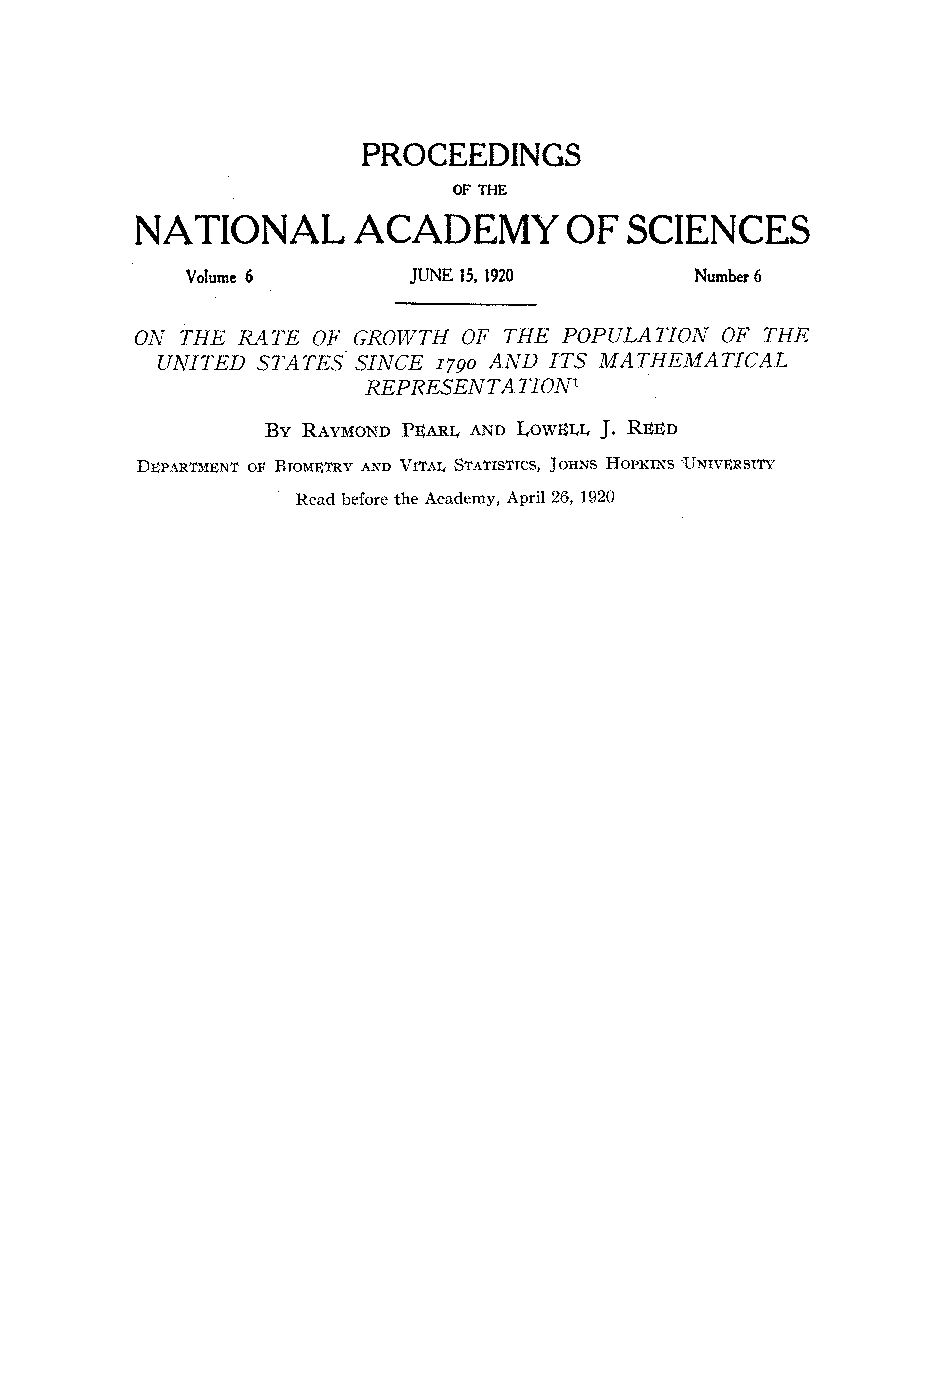
\includegraphics[width=\textwidth]{FIGS/title_PearlReed1920PNAS6}
\end{center}
}



\maxFrameImage{FIGS/table_PearlReed1920PNAS6}

\frame{\frametitle{USA census from 1790 to 1910}
Although we have data up to 2020, we use the data up to 1910 like Pearl \& Reed (note that there were some corrections to the census since the paper of Pearl \& Reed)
\vfill
\begin{center}
\begin{table}

\centering
\begin{tabular}[t]{rl}
\toprule
Year & Population\\
\midrule
1790 & 3,929,326\\
1800 & 5,308,483\\
1810 & 7,239,881\\
1820 & 9,638,453\\
1830 & 12,866,020\\
\bottomrule
\end{tabular}
\centering
\begin{tabular}[t]{rl}
\toprule
Year & Population\\
\midrule
1840 & 17,069,458\\
1850 & 23,191,876\\
1860 & 31,443,321\\
1870 & 39,818,449\\
1880 & 50,189,209\\
\bottomrule
\end{tabular}
\centering
\begin{tabular}[t]{rl}
\toprule
Year & Population\\
\midrule
1890 & 62,947,714\\
1900 & 76,212,168\\
1910 & 92,228,496\\
\bottomrule
\end{tabular}
\end{table}\end{center}
}


\begin{frame}[fragile]
\frametitle{Plot the data !!!}
It is always a good idea to plot the data before trying to do anything with it
\vfill
\begin{lstlisting}
plot_USA_census_to_1910 = 
  ggplot(USA_census_to_1910, aes(x=Year, y=Population)) +
  geom_line() +
  geom_point() +
  labs(title="US population from 1790 to 1910",
       x="Year",
       y="Population") +
  theme_minimal()
print(plot_USA_census_to_1910)
\end{lstlisting}
\end{frame}


\maxFrameImage{FIGS/slides-02-plot-census-1910-ggplot.pdf}



%%%%%%%%%%%%%%%%%%%
%%%%%%%%%%%%%%%%%%%
%%%%%%%%%%%%%%%%%%%
%%%%%%%%%%%%%%%%%%%
\section{Fitting a curve to the data}
% The section page
\newSectionSlide{FIGS/population-models-Gemini_Generated_Image_w3izodw3izodw3iz.jpeg}



%%%%%%%%%%%%%%%%%%%
%%%%%%%%%%%%%%%%%%%
\subsection{Fitting a quadratic curve to the data}
% The section page
\newSubSectionSlide{FIGS/population-models-Gemini_Generated_Image_wuhpggwuhpggwuhp.jpeg}



\frame{\frametitle{First idea -- This looks quadratic!}
The curve looks like a piece of a parabola. So let us ``fit'' a curve of the form
\[
P(t)=a+bt+ct^2
\]
\vfill
This means we want to find coefficients $a,b,c$ such that the curve $P(t)$ is as close as possible to the data points
}

\frame{\frametitle{The data points}
\begin{center}
\begin{table}

\centering
\begin{tabular}[t]{rl}
\toprule
Year & Population\\
\midrule
1790 & 3,929,326\\
1800 & 5,308,483\\
1810 & 7,239,881\\
1820 & 9,638,453\\
1830 & 12,866,020\\
\bottomrule
\end{tabular}
\centering
\begin{tabular}[t]{rl}
\toprule
Year & Population\\
\midrule
1840 & 17,069,458\\
1850 & 23,191,876\\
1860 & 31,443,321\\
1870 & 39,818,449\\
1880 & 50,189,209\\
\bottomrule
\end{tabular}
\centering
\begin{tabular}[t]{rl}
\toprule
Year & Population\\
\midrule
1890 & 62,947,714\\
1900 & 76,212,168\\
1910 & 92,228,496\\
\bottomrule
\end{tabular}
\end{table}\end{center}
\vfill
We have 13 data points $(t_k,P_k)$, $k=1,\ldots,13$, e.g., $(t_1,P_1)=(1790,3929214)$, $(t_2,P_2)=(1800,5308483)$, etc.
}


\begin{frame}{Some of you are familiar with this problem}
If you have taken MATH 2740 (Math of Data Science), you have seen this before!
\vfill
See the notes on the course website for a refresher on this problem \href{https://julien-arino.github.io/math-of-data-science/SLIDES/MATH2740-slides-04-Canada-census.html}{here} and the corresponding videos \href{https://youtu.be/c8MCbAL0NFs?si=e2Q8ZgkKEyooHpo3}{here}, \href{https://youtu.be/9hJchea1j8o?si=q-5ZM2sOUu5DSmKu}{here}, \href{https://youtu.be/3_6HEY4CmbA?si=xAcLjKS86C4FMUCp}{here}, \href{https://youtu.be/yT7aGJfRWBA?si=GrVC0mKkUkE-W2s0}{here} and \href{https://youtu.be/v-z-QaUwdEo?si=RQ6dZYAXz_68Vi-9}{here}
\vfill
(Sorry about the number of videos, I need to reorganize them!)
\end{frame}

\begin{frame}
To do this, we want to minimize
\[
S=\sum_{k=1}^{13} \left(P(t_k)-P_k\right)^2
\]
where $t_k$ are the known dates, $P_k$ are the known populations, and $P(t_k)=a+bt_k+ct_k^2$
\vfill
The $t_k$ and $P_k$ are known, $a,b,c$ are to be found, so we write $S$ as a function of $a,b,c$: $S(a,b,c)$
\end{frame}



\frame{
Recall your multivariable calculus:
\[
S=S(a,b,c)=\sum_{k=1}^{13} \left(a+bt_k+ct_k^2-P_k\right)^2
\]
is maximal if (necessary condition) $\partial S/\partial a=\partial S/\partial b=\partial S/\partial c=0$ 
}

\begin{frame}
We have
\begin{align*}
\frac{\partial S}{\partial a} &= 2\sum_{k=1}^{13}(a+bt_k+ct_k^2-P_k) \\
\frac{\partial S}{\partial b} &= 2\sum_{k=1}^{13}(a+bt_k+ct_k^2-P_k)t_k \\
\frac{\partial S}{\partial c} &= 2\sum_{k=1}^{13}(a+bt_k+ct_k^2-P_k)t_k^2
\end{align*}
\end{frame}

\frame{
Thus, we want
\begin{align*}
\frac{\partial S}{\partial a} = 0 &\iff
2\sum\textstyle{_{k=1}^{13}}(a+bt_k+ct_k^2-P_k) = 0\\
\frac{\partial S}{\partial b} = 0 &\iff
2\sum\textstyle{_{k=1}^{13}}(a+bt_k+ct_k^2-P_k)t_k = 0 \\
\frac{\partial S}{\partial c} = 0 &\iff
2\sum\textstyle{_{k=1}^{13}}(a+bt_k+ct_k^2-P_k)t_k^2 = 0,
\end{align*}
that is
\begin{align*}
\sum\textstyle{_{k=1}^{13}}(a+bt_k+ct_k^2-P_k) &= 0\\
\sum\textstyle{_{k=1}^{13}}(a+bt_k+ct_k^2-P_k)t_k &= 0 \\
\sum\textstyle{_{k=1}^{13}}(a+bt_k+ct_k^2-P_k)t_k^2 &= 0.
\end{align*}
}

\frame{
Rearranging the system
\begin{align*}
\sum\textstyle{_{k=1}^{13}}(a+bt_k+ct_k^2-P_k) &= 0\\
\sum\textstyle{_{k=1}^{13}}(a+bt_k+ct_k^2-P_k)t_k &= 0 \\
\sum\textstyle{_{k=1}^{13}}(a+bt_k+ct_k^2-P_k)t_k^2 &= 0,
\end{align*}
we get
\begin{align*}
\sum\textstyle{_{k=1}^{13}}(a+bt_k+ct_k^2) &= \sum\textstyle{_{k=1}^{13}}P_k\\
\sum\textstyle{_{k=1}^{13}}(at_k+bt_k^2+ct_k^3) &= \sum\textstyle{_{k=1}^{13}}P_kt_k\\
\sum\textstyle{_{k=1}^{13}}(at_k^2+bt_k^3+ct_k^4) &= \sum\textstyle{_{k=1}^{13}}P_kt_k^2.
\end{align*}
}

\frame{
\begin{align*}
\sum\textstyle{_{k=1}^{13}}(a+bt_k+ct_k^2) &= \sum\textstyle{_{k=1}^{13}}P_k\\
\sum\textstyle{_{k=1}^{13}}(at_k+bt_k^2+ct_k^3) &= \sum\textstyle{_{k=1}^{13}}P_kt_k\\
\sum\textstyle{_{k=1}^{13}}(at_k^2+bt_k^3+ct_k^4) &= \sum\textstyle{_{k=1}^{13}}P_kt_k^2,
\end{align*}
after a bit of tidying up, takes the form
\begin{align*}
\left(\sum_{k=1}^{13}1\right)a+\left(\sum_{k=1}^{13}t_k\right)b+\left(\sum_{k=1}^{13}t_k^2\right)c &= \sum_{k=1}^{13}P_k \\
\left(\sum_{k=1}^{13}t_k\right)a+\left(\sum_{k=1}^{13}t_k^2\right)b+\left(\sum_{k=1}^{13}t_k^3\right)c &= \sum_{k=1}^{13}P_kt_k \\
\left(\sum_{k=1}^{13}t_k^2\right)a+\left(\sum_{k=1}^{13}t_k^3\right)b+\left(\sum_{k=1}^{13}t_k^4\right)c &= \sum_{k=1}^{13}P_kt_k^2.
\end{align*}
}

\frame{
So the aim is to solve the linear system
\[
\begin{pmatrix}
13 & \sum\limits_{k=1}^{13}t_k & \sum\limits_{k=1}^{13}t_k^2 \\
\sum\limits_{k=1}^{13}t_k & \sum\limits_{k=1}^{13}t_k^2 & \sum\limits_{k=1}^{13}t_k^3 \\
\sum\limits_{k=1}^{13}t_k^2 & \sum\limits_{k=1}^{13}t_k^3 & \sum\limits_{k=1}^{13}t_k^4
\end{pmatrix}
\begin{pmatrix}
a\\ b\\ c
\end{pmatrix}
=
\begin{pmatrix}
\sum\limits_{k=1}^{13}P_k \\
\sum\limits_{k=1}^{13}P_kt_k \\
\sum\limits_{k=1}^{13}P_kt_k^2
\end{pmatrix}
\]
}

\frame[containsverbatim]{
With \code{R}, this is easy to solve
}

\frame[containsverbatim]{
Thus, to set up the problem in the form of solving $Ax=b$, we need to do the following:
\begin{verbatim}
format long g;
A=[13,sum(t),sum(t.^2);sum(t),sum(t.^2),sum(t.^3);...
sum(t.^2),sum(t.^3),sum(t.^4)];
b=[sum(P);sum(P.*t);sum(P.*(t.^2))];
\end{verbatim}
The {\tt format long g} command is used to force the display of digits (normally, what is shown is in ``scientific'' notation, not very informative here).
}

\frame[containsverbatim]{
Then, solve the system using
\begin{verbatim}
A\b
\end{verbatim}
We get the following output:
\begin{verbatim}
>> A\b
Warning: Matrix is close to singular or badly scaled.
         Results may be inaccurate. RCOND = 1.118391e-020.

ans =

        22233186177.8195
        -24720291.325476
        6872.99686313725
\end{verbatim}
(note that here, Octave gives a solution that is not as good as this one, provided by MatLab).
}


%%%%%%%%%%%%%%%%%%%
%%%%%%%%%%%%%%%%%%%
\subsection{Checking our results for the quadratic}
% The section page
\newSubSectionSlide{FIGS/population-models-Gemini_Generated_Image_w3izoew3izoew3iz.jpeg}


\frame[containsverbatim]{
Thus
\[
P(t)=22233186177.8195-24720291.325476t+6872.99686313725t^2
\]
To see what this looks like,
\begin{verbatim}
plot(t,22233186177.8195-24720291.325476.*t...
+6872.99686313725.*t.^2);
\end{verbatim}
(note the dots before multiplication and power, since we apply this function to every entry of $t$).
In fact, to compare with original data:
\begin{verbatim}
plot(t,22233186177.8195-24720291.325476.*t...
+6872.99686313725.*t.^2,t,P,'*');
\end{verbatim}
}

\maxFrameImage{FIGS/quadratic_fit}




\frame[containsverbatim]{
Form the vector of errors, and compute sum of errors squared:
\begin{verbatim}
octave:26> E=f(t)-P;
octave:27> sum(E.^2)
ans =     12186176863781.4
\end{verbatim}
Quite a large error (12,186,176,863,781.4), which is normal since we have used actual numbers, not thousands or millions of individuals, and we are taking the square of the error.
}

\frame[containsverbatim]{\frametitle{Now for the big question...}
How does our formula do for present times?
\begin{verbatim}
f(2006)
ans =     301468584.066013
\end{verbatim}
Actually, quite well: 301,468,584, compared to the 298,444,215 July 2006 estimate, overestimates the population by 3,024,369, a relative error of approximately 1\%.
}

\frame{\frametitle{The US population from 1790 to 2020 (revised numbers)}
\begin{center}
\begin{table}

\centering
\begin{tabular}[t]{rl}
\toprule
Year & Population\\
\midrule
1790 & 3,929,326\\
1800 & 5,308,483\\
1810 & 7,239,881\\
1820 & 9,638,453\\
1830 & 12,866,020\\
\addlinespace
1840 & 17,069,458\\
1850 & 23,191,876\\
1860 & 31,443,321\\
1870 & 39,818,449\\
1880 & 50,189,209\\
\bottomrule
\end{tabular}
\centering
\begin{tabular}[t]{rl}
\toprule
Year & Population\\
\midrule
1890 & 62,947,714\\
1900 & 76,212,168\\
1910 & 92,228,496\\
1920 & 106,021,537\\
1930 & 122,775,046\\
\addlinespace
1940 & 132,164,569\\
1950 & 150,697,361\\
1960 & 179,323,175\\
1970 & 203,302,031\\
1980 & 226,545,805\\
\bottomrule
\end{tabular}
\centering
\begin{tabular}[t]{rl}
\toprule
Year & Population\\
\midrule
1990 & 248,709,873\\
2000 & 281,421,906\\
2010 & 308,745,538\\
2020 & 331,449,281\\
\bottomrule
\end{tabular}
\end{table}\end{center}
}



\maxFrameImage{FIGS/slides-02-plot-census-ggplot.pdf}



%%%%%%%%%%%%%%%%%%%
%%%%%%%%%%%%%%%%%%%
\subsection{Some similar curves}
% The section page
\newSubSectionSlide{FIGS/population-models-Gemini_Generated_Image_8z3li8z3li8z3li8.jpeg}

\frame{\frametitle{Other similar approaches}
Pritchett, 1891:
\[
P=a+bt+ct^2+dt^3.
\]
(we have done this one, and found it to be quite good too).\\
Pearl, 1907:
\[
P(t)=a+bt+ct^2+d\ln t.
\]
Finds
\[
P(t)=9,064,900-6,281,430t+842,377t^2+19,829,500\ln t.
\]
}

\maxFrameImage{FIGS/table2_PearlReed1920PNAS6}



%%%%%%%%%%%%%%%%%%%
%%%%%%%%%%%%%%%%%%%
\subsection{Other population curves}
% The section page
\newSubSectionSlide{FIGS/population-models-Gemini_Generated_Image_w3izofw3izofw3iz.jpeg}


\frame{\frametitle{The logistic curve}
Pearl and Reed try
\[
P(t)=\frac{be^{at}}{1+ce^{at}}
\]
or
\[
P(t)=\frac{b}{e^{-at}+c}.
\]
%They find
%\[
%P(t)=\frac{2,930.3009}{e^{-0.0313395t}+0.014854}.
%\]
}


\frame{\frametitle{What is wrong with the logistic equation here?}
\begin{itemize}
\item The carrying capacity is constant.
\item The model does not take immigration into account (for the US, this is an important component).
\end{itemize}
}


\subsection{Population curves -- Gompertz}

\maxFrameImage{FIGS/title_Winsor1932PNAS18}
\maxFrameImage{FIGS/table_Winsor1932PNAS18}


%%%%%%%%%%%%%%%%%%%%%
%%%%%%%%%%%%%%%%%%%%%
%%%%%%%%%%%%%%%%%%%%%
%%%%%%%%%%%%%%%%%%%%%
\section{Least squares problems}

\begin{frame}{A.k.a. if the Math Dept was less \#\$\%\&, you'd know this}
	The following are a brief extract from MATH 2740 slides...
\end{frame}


\begin{frame}{The least squares problem (simplest version)}
	\begin{definition}
		Given a collection of points $(x_1,y_1),\ldots,(x_n,y_n)$, find the coefficients $a,b$ of the line $y=a+bx$ such that
		$$
		\|\mathbf{e}\|=\sqrt{\varepsilon_1^2+\cdots+\varepsilon_n^2}
		=\sqrt{(y_1-\tilde y_1)^2+\cdots+(y_n-\tilde y_n)^2}
		$$
		is minimal, where $\tilde y_i=a+bx_i$ for $i=1,\ldots,n$
	\end{definition}
	\vfill
	We just saw how to solve this by brute force using a genetic algorith to minimise $\|e\|$, let us now see how to solve this problem ``properly''
\end{frame}


\begin{frame}
	For a data point $i=1,\ldots,n$
	\[
	\varepsilon_i = y_i-\tilde y_i = y_i - (a+bx_i)
	\]
	So if we write this for all data points,
	\begin{align*}
	\varepsilon_1 &= y_1 - (a+bx_1) \\
	&\;\;\vdots \\
	\varepsilon_n &= y_n - (a+bx_n) \\
	\end{align*}
	In matrix form
	\[
	\be = \bb-A\bx
	\]
	with
	\[
	\be = \begin{pmatrix}
	\varepsilon_1\\ \vdots\\ \varepsilon_n
	\end{pmatrix},
	A=\begin{pmatrix}
	1 & x_1 \\ \vdots & \vdots \\ 1 & x_n
	\end{pmatrix},
	\bx = \begin{pmatrix}
	a\\b
	\end{pmatrix}\textrm{ and }
	\bb = \begin{pmatrix}
	y_1\\ \vdots\\ y_n
	\end{pmatrix}
	\]
\end{frame}

\begin{frame}{The least squares problem (reformulated)}
\begin{definition}[Least squares solutions]
Consider a collection of points $(x_1,y_1),\ldots,(x_n,y_n)$, a matrix $A\in\M_{mn}$, $\bb\in\IR^m$. A \textbf{least squares solution} of $A\bx=\bb$ is a vector $\tilde \bx\in\IR^n$ s.t.
\[
\forall \bx\in\IR^n,\quad \|\bb-A\tilde\bx\|\leq \|\bb-A\bx\|
\]
\end{definition}
\end{frame}


\begin{frame}{Needed to solve the problem}
\begin{definition}[Best approximation]
Let $V$ be a vector space, $W\subset V$ and $\mathbf{v}\in V$. The \textbf{best approximation} to $\mathbf{v}$ in $W$ is $\tilde{\mathbf{v}}\in W$ s.t.
\[
\forall\mathbf{w}\in W, \mathbf{w}\neq\tilde{\mathbf{v}}, \quad
\|\mathbf{v}-\tilde{\mathbf{v}}\| < \|\mathbf{v}-\mathbf{w}\|
\]
\end{definition}
\vfill
\begin{theorem}[Best approximation theorem]
Let $V$ be a vector space with an inner product, $W\subset V$ and $\mathbf{v}\in V$. Then $\mathsf{proj}_W(\mathbf{v})$ is the best approximation to $\mathbf{v}$ in W
\end{theorem}
\end{frame}


\begin{frame}{Let us find the least squares solution}
$\forall \bx\IR^n$, $A\bx$ is a vector in the \textbf{column space} of $A$ (the space spanned by the vectors making up the columns of $A$)
\vfill
Since $\bx\in\IR^n$, $A\bx\in\mathsf{col}(A)$
\vfill
$\implies$ least squares solution of $A\bx=\bb$ is a vector $\tilde\by\in\mathsf{col}(A)$ s.t.
\[
\forall\by\in\mathsf{col}(A),\quad\|\bb-\tilde\by\|\leq\|\bb-\by\|
\]
\vfill
This looks very much like Best approximation and Best approximation theorem
\end{frame}

\begin{frame}{Putting things together}
We just stated: The least squares solution of $A\bx=\bb$ is a vector $\tilde\by\in\mathsf{col}(A)$ s.t.
\[
\forall\by\in\mathsf{col}(A),\quad\|\bb-\tilde\by\|\leq\|\bb-\by\|
\]
\vfill
We know (reformulating a tad):
\begin{theorem}[Best approximation theorem]
Let $V$ be a vector space with an inner product, $W\subset V$ and $\mathbf{v}\in V$. Then $\mathsf{proj}_W(\mathbf{v})\in W$ is the best approximation to $\mathbf{v}$ in W, i.e.,
\[
\forall\mathbf{w}\in W, \mathbf{w}\neq\mathsf{proj}_W(\mathbf{v}), \quad
\|\mathbf{v}-\mathsf{proj}_W(\mathbf{v})\| < \|\mathbf{v}-\mathbf{w}\|
\]
\end{theorem}
\vfill
$\implies$ $W=\mathsf{col}(A)$, $\bv=\bb$ and $\tilde\by=\mathsf{proj}_{\mathsf{col}(A)}(\mathbf{b})$
\end{frame}

\begin{frame}
So if $\tilde\bx$ is a least squares solution of $A\bx=\bb$, then
\[
\tilde\by = A\tilde\bx = \mathsf{proj}_{\mathsf{col}(A)}(\mathbf{b})
\]
\vfill
We have
\[
\bb-A\tilde\bx = \bb-\mathsf{proj}_{\mathsf{col}(A)}(\mathbf{b}) 
= \mathsf{perp}_{\mathsf{col}(A)}(\mathbf{b})
\]
and it is easy to show that
\[
\mathsf{perp}_{\mathsf{col}(A)}(\mathbf{b}) \perp \mathsf{col}(A)
\]
\vfill
So for all columns $\ba_i$ of $A$
\[
\ba_i\boldsymbol{\cdot}(\bb-A\tilde\bx) = 0
\]
which we can also write as $\ba_i^T(\bb-A\tilde\bx) = 0$
\end{frame}

\begin{frame}
For all columns $\ba_i$ of $A$,
\[\ba_i^T(\bb-A\tilde\bx) = 0
\]
\vfill
This is equivalent to saying that
\[
A^T(\bb-A\tilde\bx) = \b0
\]
\vfill
We have
\begin{align*}
A^T(\bb-A\tilde\bx) = \b0 &\iff A^T\bb - A^TA\tilde\bx = \b0 \\
&\iff A^T\bb = A^TA\tilde\bx \\
&\iff A^TA\tilde\bx = A^T\bb
\end{align*}
The latter system constitutes the \textbf{normal equations} for $\tilde\bx$
\end{frame}


\begin{frame}{Least squares theorem}
\begin{importanttheorem}[Least squares theorem]\label{th:least_squares}
$A\in\M_{mn}$, $\bb\in\IR^m$. Then
\begin{enumerate}
\item $A\bx=\bb$ always has at least one least squares solution $\tilde\bx$
\item $\tilde\bx$ least squares solution to $A\bx=\bb$ $\iff$ $\tilde\bx$ is a solution to the normal equations $A^TA\tilde\bx = A^T\bb$
\item $A$ has linearly independent columns $\iff$ $A^TA$ invertible.  
\newline In this case, the least squares solution is unique and 
\[
\tilde\bx = \left(A^TA\right)^{-1}A^T\bb
\]
\end{enumerate}
\end{importanttheorem}
\vfill
We have seen 1 and 2, we will not show 3 (it is not hard)
\end{frame}


\subsection{Fitting something more complicated}

\begin{frame}{Suppose we want to fit something a bit more complicated..}
For instance, instead of the affine function
\[
y = a+bx
\]
suppose we want to do the quadratic
\[
y = a_0+a_1x+a_2x^2
\]
or even
\[
y = k_0 e^{k_1x}
\]
\vfill
How do we proceed?
\end{frame}


\begin{frame}{Fitting the quadratic}
We have the data points $(x_1,y_1),(x_2,y_2),\ldots,(x_n,y_n)$ and want to fit
\[
y = a_0+a_1x+a_2x^2
\]
At $(x_1,y_1)$,
\[
\tilde y_1 = a_0+a_1x_1+a_2x_1^2
\]
$\vdots$\\
At $(x_n,y_n)$,
\[
\tilde y_n = a_0+a_1x_n+a_2x_n^2
\]
\end{frame}

\begin{frame}
In terms of the error
\begin{align*}
\varepsilon_1 &= y_1-\tilde y_1 = y_1-(a_0+a_1x_1+a_2x_1^2) \\
&\;\;\vdots\\
\varepsilon_n &= y_n-\tilde y_n = y_n-(a_0+a_1x_n+a_2x_n^2)
\end{align*}
i.e.,
\[
\be = \bb-A\bx 
\]
where
\[
\be = \begin{pmatrix}
\varepsilon_1\\ \vdots\\ \varepsilon_n
\end{pmatrix},
A=\begin{pmatrix}
1 & x_1 & x_1^2\\ \vdots & \vdots & \vdots \\ 1 & x_n & x_n^2
\end{pmatrix},
\bx = \begin{pmatrix}
a_0\\a_1\\a_2
\end{pmatrix}\textrm{ and }
\bb = \begin{pmatrix}
y_1\\ \vdots\\ y_n
\end{pmatrix}
\]
\vfill
Theorem~\ref{th:least_squares} applies, with here $A\in\M_{n3}$ and $\bb\in\IR^n$
\end{frame}


\begin{frame}{Fitting the exponential}
Things are a bit more complicated here
\vfill
If we proceed as before, we get the system
\begin{align*}
y_1 &= k_0 e^{k_1x_1} \\
&\;\;\vdots \\
y_n &= k_0 e^{k_1x_n}
\end{align*}
$e^{k_1x_i}$ is a nonlinear term, it cannot be put in a matrix
\vfill
\emph{However}: take the $\ln$ of both sides of the equation
\[
\ln(y_i) = \ln(k_0e^{k_1x_i}) = \ln(k_0)+\ln(e^{k_1x_i}) = \ln(k_0)+k_1x_i
\]
If $y_i,k_0>0$, then their $\ln$ are defined and we're in business..
\end{frame}

\begin{frame}
\[
\ln(y_i) = \ln (k_0)+k_1x_i
\]
So the system is
\begin{align*}
\by = A\bx+\bb
\end{align*}
with
\[
A = \begin{pmatrix}
x_1\\ \vdots \\ x_n
\end{pmatrix},
\bx = \begin{pmatrix}
k_1
\end{pmatrix},
\bb = \begin{pmatrix}
\ln (k_0)
\end{pmatrix}
\textrm{ and }
\by = \begin{pmatrix}
\ln (y_1)\\ \vdots\\ \ln (y_n)
\end{pmatrix}
\]
\end{frame}


%%%%%%%%%%%%%%%%%%%
%%%%%%%%%%%%%%%%%%%
%%%%%%%%%%%%%%%%%%%
%%%%%%%%%%%%%%%%%%%
\section{Population growth -- Logistic equation}
% The section page
\newSectionSlide{FIGS/population-models-Gemini_Generated_Image_gsewj8gsewj8gsew.jpeg}


\frame{\frametitle{The logistic equation}
The logistic curve is the solution to the ordinary differential equation
\[
N'=rN\left(1-\frac NK\right),
\]
which is called the \textbf{logistic equation}. $r$ is the \textbf{intrinsic growth rate}, $K$ is the \textbf{carrying capacity}.
\vskip1cm
This equation was introduced by Pierre-Fran\c{c}ois Verhulst (1804-1849), in 1844.
}

\frame{\frametitle{Deriving the logistic equation}
The idea is to represent a population with the following components:
\begin{itemize}
\item birth, at the \textbf{per capita} rate $b$,
\item death, at the \textbf{per capita} rate $d$,
\item competition of individuals with other individuals reduces their ability to survive, resulting in death.
\end{itemize}
This gives
\[
N'=bN-dN-\textrm{competition}.
\]
}

\frame{\frametitle{Accounting for competition}
Competition describes the mortality that occurs when two individuals meet.
\begin{itemize}
\item
In chemistry, if there is a concentration $X$ of one product and $Y$ of another product, then $XY$, called \textbf{mass action}, describes the number of interactions of molecules of the two products.
\item
Here, we assume that $X$ and $Y$ are of the same type (individuals). So there are $N^2$ contacts.
\item
These $N^2$ contacts lead to death of one of the individuals at the rate $c$.
\end{itemize}
Therefore, the \textbf{logistic} equation is
\[
N'=bN-dN-cN^2.
\]
}

\frame{\frametitle{Reinterpreting the logistic equation}
The equation
\[
N'=bN-dN-cN^2
\]
is rewritten as
\[
N'=(b-d)N-cN^2.
\]
\begin{itemize}
\item $b-d$ represents the rate at which the population increases (or decreases) in the absence of competition. It is called the \textbf{intrinsic growth rate} of the population.
\item $c$ is the rate of \textbf{intraspecific} competition. The prefix \textbf{intra} refers to the fact that the competition is occurring between members of the same species, that is, within the species.\newline
[We will see later examples of \textbf{interspecific} competition, that is, between different species.]
\end{itemize}
}


\frame{\frametitle{Another (..) interpretation of the logistic equation}
We have
\[
N'=(b-d)N-cN^2.
\]
Factor out an $N$:
\[
N'=\bigl((b-d)-cN\bigr)N.
\]
This gives us another interpretation of the logistic equation. Writing
\[
\frac{N'}N=(b-d)-cN,
\]
we have $N'/N$, the \textbf{per capita growth rate} of $N$, given by a constant, $b-d$, minus a \textbf{density dependent inhibition} factor, $cN$.
}

\frame{\frametitle{Equivalent equations}
\begin{align*}
N' &= (b-d)N-cN^2\\
&= \bigl((b-d)-cN\bigr)N \\
&= \left(r-\frac rr cN\right)N,\quad\textrm{with }r=b-d \\
&= rN\left(1-\frac crN\right) \\
&= rN\left(1-\frac NK\right),
\end{align*}
with
\[
\frac cr=\frac 1K,
\]
that is, $K=r/c$.
}

\frame{\frametitle{3 ways to tackle this equation}
\begin{enumerate}
\item The equation is separable. [explicit method]
\item The equation is a Bernoulli equation. [explicit method]
\item Use qualitative analysis.
\end{enumerate}
}


%%%%%%%%%%%%%%%%%%%
%%%%%%%%%%%%%%%%%%%
%%%%%%%%%%%%%%%%%%%
%%%%%%%%%%%%%%%%%%%
\subsection{Qualitative analysis of the logistic equation}
% The section page
\newSubSectionSlide{FIGS/population-models-Gemini_Generated_Image_8z3lj8z3lj8z3lj8.jpeg}



\frame{\frametitle{Studying the logistic equation qualitatively}
We study
\begin{equation}\label{eq:logistic_ode}
N'=rN\left(1-\frac NK\right).\tag{ODE1}
\end{equation}
For this, write
\[
f(N)=rN\left(1-\frac NK\right).
\]
Consider the initial value problem (IVP)
\begin{equation}\label{ivp:logistic_ode}
N'=f(N),\quad N(0)=N_0>0.\tag{IVP1}
\end{equation}
\begin{itemize}
\item $f$ is $C^1$ (differentiable with continuous derivative) so solutions to \eqref{ivp:logistic_ode} exist and are unique.
\end{itemize}
}

\frame{
\textbf{Equilibria} of \eqref{eq:logistic_ode} are points such that $f(N)=0$ (so that $N'=f(N)=0$, meaning $N$ does not vary). So we solve $f(N)=0$ for $N$. We find two points:
\begin{itemize}
\item $N=0$
\item $N=K$.
\end{itemize}
By uniqueness of solutions to \eqref{ivp:logistic_ode}, solutions cannot cross the lines $N(t)=0$ and $N(t)=K$.
}

\frame{
There are several cases.
\begin{itemize}
\item $N=0$ for some $t$, then $N(t)=0$ for all $t\geq 0$, by uniqueness of solutions.
\item $N\in(0,K)$, then $rN>0$ and $N/K<1$ so $1-N/K>0$, which implies that $f(N)>0$. As a consequence, $N(t)$ increases if $N\in(0,K)$.
\item $N=K$, then $rN>0$ but $N/K=1$ so $1-N/K=0$, which implies that $f(N)=0$. As a consequence, $N(t)=K$ for all $t\geq 0$, by uniqueness of solutions.
\item $N>K$, the $rN>0$ and $N/K>1$, implying that $1-N/K<0$ and in turn, $f(N)<0$. As a consequence, $N(t)$ decreases if $N\in(K,+\infty)$.
\end{itemize}
}

\frame{
Therefore,
\begin{theorem}
Suppose that $N_0>0$. Then the solution $N(t)$ of \eqref{ivp:logistic_ode} is such that
\[
\lim_{t\to\infty} N(t)=K,
\]
so that $K$ is the number of individuals that the environment can support, the \textbf{carrying capacity} of the environment.

If $N_0=0$, then $N(t)=0$ for all $t\geq 0$.
\end{theorem}
}


%%%%%%%%%%%%%%%%%%%
%%%%%%%%%%%%%%%%%%%
%%%%%%%%%%%%%%%%%%%
%%%%%%%%%%%%%%%%%%%
\section{The delayed logistic equation}
% The section page
\newSectionSlide{FIGS/population-models-Gemini_Generated_Image_hc77fbhc77fbhc77.jpeg}




\frame{\frametitle{The delayed logistic equation}
Consider the equation as
\[
\frac{N'}{N}=(b-d)-cN,
\]
that is, the per capita rate of growth of the population depends on the net growth rate $b-d$, and some density dependent inhibition $cN$ (resulting of competition).
\vskip0.5cm
Suppose that instead of instantaneous inhibition, there is some delay $\tau$ between the time the inhibiting event takes place and the moment when it affects the growth rate.
\vskip0.5cm
For example, two individuals fight for food, and one later dies of the injuries sustained during this fight.
}

\frame{\frametitle{The delayed logistic equation}
In the case of a time $\tau$ between inhibiting event and inhibition, the equation would be written as
\[
\frac{N'}N=(b-d)-cN(t-\tau).
\]
Using the change of variables introduced earlier, this is written
\begin{equation}\label{eq:logistic_dde}
N'(t)=rN(t)\left(1-\frac{N(t-\tau)}K\right). \tag{DDE1}
\end{equation}
Such an equation is called a \textbf{delay} differential equation. It is much more complicated to study than \eqref{eq:logistic_ode}. In fact, some things remain unknown about \eqref{eq:logistic_dde}.
}

\frame{\frametitle{Delayed initial value problem}
The IVP takes the form
\begin{equation}\label{ivp:logistic_dde}
\begin{aligned}
N'(t)&= rN(t)\left(1-\frac{N(t-\tau)}K\right),\\
N(t) &= \phi(t)\textrm{ for }t\in[-\tau,0],
\end{aligned} \tag{IVP2}
\end{equation}
where $\phi(t)$ is some continuous function. Hence, initial conditions (called initial data in this case) must be specified on an interval, instead of being specified at a point, to guarantee existence and uniqueness of solutions.

We will not learn how to study this type of equation (this is graduate level mathematics). I will give a few results.
}

\frame{
To find equilibria, remark that delay should not play a role, since $N$ should be constant. Thus, equilibria are found by considering the equation with no delay, which is \eqref{eq:logistic_ode}.
\begin{theorem}
Suppose that $r\tau<\pi/2$. Then solutions of \eqref{ivp:logistic_dde} with positive initial data $\phi(t)$ starting close enough to $K$ tend to $K$. If $r\tau<37/24$, then all solutions of  \eqref{ivp:logistic_dde} with positive initial data $\phi(t)$ tend to $K$. If $r\tau>\pi/2$, then $K$ is an unstable equilibrium and all solutions of \eqref{ivp:logistic_dde} with positive initial data $\phi(t)$ on $[-\tau,0]$ are oscillatory.
\end{theorem}
\vskip1cm

There is a gray zone between $37/24$ ($\simeq 1.5417$) and $\pi/2$ ($\simeq 1.5708$). The global aspect was proved for $r\tau<37/24$ in 1945 by Wright. Although there is very strong numerical evidence that this is in fact true up to $\pi/2$, nobody has yet managed to prove it.
}



%%%%%%%%%%%%%%%%%%%
%%%%%%%%%%%%%%%%%%%
%%%%%%%%%%%%%%%%%%%
%%%%%%%%%%%%%%%%%%%
\section{The logistic map}
% The section page
\newSectionSlide{FIGS/population-models-Gemini_Generated_Image_x4kl2ox4kl2ox4kl.jpeg}



\frame{\frametitle{Discrete-time systems}
So far, we have seen continuous-time models, where $t\in\IR_+$. Another way to model natural phenomena is by using a discrete-time formalism, that is, to consider equations of the form
\[
x_{t+1}=f(x_t),
\]
where $t\in\IN$ or $\IZ$, that is, $t$ takes values in a discrete valued (countable) set.
\vskip0.5cm
Time could for example be days, years, etc.
}


\frame{\frametitle{The logistic map}
The logistic \textbf{map} is, for $t\geq 0$,
\begin{equation}\label{eq:logistic_discrete}
N_{t+1}=rN_t\left(1-\frac{N_t}K\right). \tag{DT1}
\end{equation}
To transform this into an initial value problem, we need to provide an initial condition $N_0\geq 0$ for $t=0$.
}


\frame{\frametitle{Some mathematical analysis}
Suppose we have a system in the form
\[
x_{t+1}=f(x_t),
\]
with initial condition given for $t=0$ by $x_0$. Then,
\begin{align*}
x_1 &= f(x_0) \\
x_2 &= f(x_1)= f(f(x_0))\stackrel{\Delta}{=} f^2(x_0) \\
& \vdots \\
x_k &= f^k(x_0).
\end{align*}
The $f^k=\underbrace{f\circ f\circ\cdots\circ f}_{k\textrm{ times}}$ are called the \textbf{iterates} of $f$.
}

\frame{\frametitle{Fixed points}
\begin{definition}[Fixed point]
Let $f$ be a function. A point $p$ such that $f(p)=p$ is called a \textbf{fixed point} of $f$.
\end{definition}
\begin{theorem}
Consider the closed interval $I=[a,b]$. If $f:I\to I$ is continuous, then $f$ has a fixed point in $I$.
\end{theorem}
\begin{theorem}
Let $I$ be a closed interval and $f:I\to\IR$ be a continuous function. If $f(I)\supset I$, then $f$ has a fixed point in $I$.
\end{theorem}
}

\frame{\frametitle{Periodic points}
\begin{definition}[Periodic point]
Let $f$ be a function. If there exists a point $p$ and an integer $n$ such that
\[
f^n(p)=p,\quad\textrm{but}\quad f^k(p)\neq p\textrm{ for }k<n,
\]
then $p$ is a periodic point of $f$ with (least) period $n$ (or a $n$-periodic point of $f$).
\end{definition}
\vskip0.5cm
Thus, $p$ is a $n$-periodic point of $f$ iff $p$ is a $1$-periodic point of $f^n$.
}


\frame{\frametitle{Stability of fixed points, of periodic points}
\begin{theorem}
Let $f$ be a continuously differentiable function (that is, differentiable with continuous derivative, or $C^1$), and $p$ be a fixed point of $f$.
\begin{enumerate}
\item If $|f'(p)|<1$, then there is an open interval $\mathcal{I}\ni p$ such that $\lim_{k\to\infty}f^k(x)=p$ for all $x\in\mathcal{I}$.
\item If $|f'(p)|>1$, then there is an open interval $\mathcal{I}\ni p$ such that if $x\in\mathcal{I}$, $x\neq p$, then there exists $k$ such that $f^k(x)\not\in\mathcal{I}$.
\end{enumerate}
\end{theorem}
\begin{definition}
Suppose that $p$ is a $n$-periodic point of $f$, with $f\in C^1$.
\begin{itemize}
\item If $|\left(f^n\right)'(p)|<1$, then $p$ is an \textbf{attracting} periodic point of $f$.
\item If $|\left(f^n\right)'(p)|>1$, then $p$ is an \textbf{repelling} periodic point of $f$.
\end{itemize}
\end{definition}
}

\frame{\frametitle{Parametrized families of functions}
Consider the equation \eqref{eq:logistic_discrete}, which for convenience we rewrite as
\begin{equation}\label{eq:logistic_discrete_scaled}
N_{t+1}=rN_t(1-N_t)\tag{DT2},
\end{equation}
where $r$ is a parameter in $\IR_+$, and $N$ will typically be taken in $[0,1]$. Let
\[
f_r(x)=rx(1-x).
\]
The function $f_r$ is called a \textbf{parametrized family} of functions.
}

\frame{\frametitle{Bifurcations}
\begin{definition}[Bifurcation]
Let $f_\mu$ be a parametrized family of functions.
Then there is a \textbf{bifurcation} at $\mu=\mu_0$ (or $\mu_0$ is a bifurcation point) if there exists $\varepsilon>0$ such that, if $\mu_0-\varepsilon<a<\mu_0$ and $\mu_0<b<\mu_0+\varepsilon$, then the dynamics of $f_a(x)$ are ``different'' from the dynamics of $f_b(x)$.
\end{definition}
\vfill
An example of ``different'' would be that $f_a$ has a fixed point (that is, a 1-periodic point) and $f_b$ has a 2-periodic point.
}


\frame{\frametitle{Back to the logistic map}
Consider the simplified version \eqref{eq:logistic_discrete_scaled},
\[
N_{t+1}=rN_t(1-N_t)\stackrel{\Delta}{=}f_r(N_t).
\]
\textbf{Are solutions well defined?}

Suppose $N_0\in[0,1]$, do we stay in $[0,1]$?
$f_r$ is continuous on $[0,1]$, so it has a extrema on $[0,1]$. We have
\[
f_r'(x)=r-2rx=r(1-2x),
\]
which implies that $f_r$ increases for $x<1/2$ and decreases for $x>1/2$, reaching a maximum at $x=1/2$.
\vfill
$f_r(0)=f_r(1)=0$ are the minimum values, and $f(1/2)=r/4$ is the maximum. Thus, if we want $N_{t+1}\in[0,1]$ for $N_t\in[0,1]$, we need to consider $r\leq 4$.
}

\frame{
\begin{itemize}
\item Note that if $N_0=0$, then $N_t=0$ for all $t\geq 1$.
\item Similarly, if $N_0=1$, then $N_1=0$, and thus $N_t=0$ for all $t\geq 1$.
\item This is true for all $t$: if there exists $t_k$ such that $N_{t_k}=1$, then $N_t=0$ for all $t\geq t_k$.
\item This last case might occur if $r=4$, as we have seen.
\item Also, if $r=0$ then $N_t=0$ for all $t$.
\end{itemize}
For these reasons, we generally consider
\[
N\in(0,1)
\]
and
\[
r\in(0,4).
\]
}

\frame{\frametitle{Fixed points: existence}
\textbf{Fixed points} of \eqref{eq:logistic_discrete_scaled} satisfy $N=rN(1-N)$, giving:
\begin{itemize}
\item $N=0$;
\item $1=r(1-N)$, that is, $p\stackrel{\Delta}{=}\dfrac{r-1}{r}$.
\end{itemize}
Note that $\lim_{r\to 0^+}p=1-\lim_{r\to 0^+}1/r=-\infty$, $\frac{\partial}{\partial r}p=1/r^2>0$ (so $p$ is an increasing function of $r$), $p=0\Leftrightarrow r=1$ and $\lim_{r\to\infty}p=1$.
So we come to this first conclusion:
\begin{itemize}
\item 0 always is a fixed point of $f_r$.
\item If $0<r<1$, then $p$ takes negative values so is not relevant.
\item If $1<r<4$, then $p$ exists.
\end{itemize}
}


\frame{\frametitle{Stability of the fixed points}
\textbf{Stability} of the fixed points is determined by the (absolute) value $f_r'$ at these fixed points. We have
\[
|f'_r(0)|=r,
\]
and
\begin{align*}
|f'_r(p)| &= \left|r-2r\dfrac{r-1}{r}\right|\\
&= |r-2(r-1)| \\
&= |2-r|
\end{align*}
Therefore, we have
\begin{itemize}
\item if $0<r<1$, then the fixed point $N=p$ does not exist and $N=0$ is attracting,
\item if $1<r<3$, then $N=0$ is repelling, and $N=p$ is attracting,
\item if $r>3$, then $N=0$ and $N=p$ are repelling.
\end{itemize}
}

\maxFrameImage{FIGS/bif_cascade_1}


\frame{\frametitle{Another bifurcation}
Thus the points $r=1$ and $r=3$ are bifurcation points. To see what happens when $r>3$, we need to look for period 2 points.

\begin{align}
f_r^2(x) &= f_r(f_r(x)) \nonumber\\
&= r f_r(x)(1-f_r(x)) \nonumber\\
&= r^2 x(1-x)(1-r x(1-x)). \label{eq:f_mu_2_a}
\end{align}
0 and $p$ are points of period 2, since a fixed point $x^*$ of $f$ satisfies $f(x^*)=x^*$, and so, $f^2(x^*)=f(f(x^*))=f(x^*)=x^*$.

This helps localizing the other periodic points. Writing the fixed point equation as
\[
Q(x)\stackrel{\Delta}{=}f_r^2(x)-x=0,
\]
we see that, since $0$ and $p$ are fixed points of $f_\mu^2$, they are roots of $Q(x)$. Therefore, $Q$ can be factorized as
\[
Q(x)=x(x-p)(-r^3x^2+Bx+C),
\]
}


\frame{
Substitute the value $(r-1)/r$ for $p$ in $Q$, develop $Q$ and \eqref{eq:f_mu_2_a} and equate coefficients of like powers gives
\begin{equation}\label{eq:Q}
Q(x)=x\left(x-\frac{r-1}{r}\right)\left(-r^3 x^2+r^2(r+1)x-r(r+1)\right).
\end{equation}
We already know that $x=0$ and $x=p$ are roots of \eqref{eq:Q}. So we search for roots of
\[
R(x):=-r^3 x^2+r^2(r+1)x-r(r+1).
\]
Discriminant is
\begin{align*}
\Delta &=r^4(r+1)^2-4r^4(r+1)\\
&= r^4(r+1)(r+1-4)\\
&= r^4(r+1)(r-3).
\end{align*}
Therefore, $R$ has distinct real roots if $r>3$.
Remark that for $r=3$, the (double) root is $p=2/3$. For $r>3$ but very close to 3, it follows from the continuity of $R$ that the roots are close to $2/3$.

}


\frame{\frametitle{Descartes' rule of signs}
\begin{theorem}[Descartes' rule of signs]\label{th:descartes}
Let $p(x) = \sum_{i=0}^m a_ix^i $ be a polynomial with real coefficients such that $a_m \neq 0$.
Define $v$ to be the number of {\it variations in sign} of the sequence of coefficients $a_m, \ldots, a_0$. By 'variations in sign' we mean the number of values of $n$ such that the sign of $a_n$ differs from the sign of $a_{n - 1}$, as $n$ ranges from $m$ down to 1.
Then
\begin{itemize}
\item the number of positive real roots of $p(x)$ is $v-2N$ for some integer $N$ satisfying $0 \leq N \leq \dfrac{v}{2}$,
\item the number of negative roots of $p(x)$ may be obtained by the same method by applying the rule of signs to $p(-x)$.
\end{itemize}
\end{theorem}
}

\frame{\frametitle{Example of use of Descartes' rule}
\begin{example}
Let
\[
p(x) = x^3+3x^2-x-3.
\]
Coefficients have signs $++--$, i.e., 1 sign change.
Thus $v = 1$. Since $0 \leq N \leq 1/2$, we must have $N=0$. Thus $v-2N=1$ and there is exactly one positive real root of $p(x)$.

To find the negative roots, we examine $p(-x) = -x^3+3x^2+x-3$. Coefficients have signs $-++-$, i.e., 2 sign changes. Thus $v=2$ and $0 \leq N \leq 2/2= 1$.
Thus, there are two possible solutions, $N=0$ and $N=1$, and two possible values of $v-2N$. Therefore, there are either two or no negative real roots.
Furthermore, note that $p(-1)=(-1)^3+3 \cdot (-1)^2-(-1)-3=0$, hence there is at least one negative root. Therefore there must be exactly two.
\end{example}
}

\frame{\frametitle{Back to the logistic map and the polynomial $R$..}
We use Descartes' rule of signs.
\begin{itemize}
\item
$R$ has signed coefficients $-+-$, so 2 sign changes imlying 0 or 2 positive real roots.
\item
$R(-x)$ has signed coefficients $---$, so no negative real roots.
\item
Since $\Delta>0$, the roots are real, and thus it follows that both roots are positive.
\end{itemize}
To show that the roots are also smaller than 1, consider the change of variables $z=x-1$. The polynomial $R$ is transformed into
\begin{align*}
R_2(z) &= -r^3 (z+1)^2+r^2(r+1)(z+1)-r(r+1) \\
&= -r^3z^2+r^2(1-r)z-r.
\end{align*}
For $r>1$, the signed coefficients are $---$, so $R_2$ has no root $z>0$, implying in turn that $R$ has no root $x>1$.
}


\frame{\frametitle{Summing up}
\begin{itemize}
\item If $0<r<1$, then $N=0$ is attracting, $p$ does not exist and there are no period 2 points.
\item At $r=1$, there is a bifurcation (called a \textbf{transcritical} bifurcation).
\item If $1<r<3$, then $N=0$ is repelling, $N=p$ is attracting, and there are no period 2 points.
\item At $r=3$, there is another bifurcation (called a \textbf{period-doubling} bifurcation).
\item For $r>3$, both $N=0$ and $N=p$ are repelling, and there is a period 2 point.
\end{itemize}
}

\maxFrameImage{FIGS/bif_cascade_2}
\maxFrameImage{FIGS/bif_cascade_3}
\maxFrameImage{FIGS/bif_cascade_4}

\frame{\frametitle{The period-doubling cascade to chaos}
The logistic map undergoes a sequence of period doubling bifurcations, called the \textbf{period-doubling cascade}, as $r$ increases from 3 to 4.

\begin{itemize}
\item Every successive bifurcation leads to a doubling of the period.
\item The bifurcation points form a sequence, $\{r_n\}$, that has the property that
\[
\lim{n\to\infty}\frac{r_n-r_{n-1}}{r_{n+1}-r_n}
\]
exists and is a constant, called the Feigenbaum constant, equal to 4.669202\ldots
\item This constant has been shown to exist in many of the maps that undergo the same type of cascade of period doubling bifurcations.
\end{itemize}
}


\frame{\frametitle{Chaos}
After a certain value of $r$, there are periodic points with all periods. In particular, there are periodic points of period 3.
\vskip1cm
By a theorem (called \textbf{Sarkovskii's theorem}), the presence of period 3 points implies the presence of points of all periods.
\vskip1cm
At this point, the system is said to be in a \textbf{chaotic regime}, or \textbf{chaotic}.
}

\maxFrameImage{FIGS/cascade_29_4}
\maxFrameImage{FIGS/cascade_full}



%%%%%%%%%%%%%%%%%%%
%%%%%%%%%%%%%%%%%%%
%%%%%%%%%%%%%%%%%%%
%%%%%%%%%%%%%%%%%%%
\section{Conclusion}
% The section page
\newSectionSlide{FIGS/population-models-Gemini_Generated_Image_8z3li8z3li8z3li8.jpeg}



\frame{\frametitle{A word of caution}
We have used three different modelling paradigms to describe the growth of a population in a \textbf{logistic} framework:
\begin{itemize}
\item The ODE version has monotone solutions converging to the carrying capacity $K$.
\item The DDE version has oscillatory solutions, either converging to $K$ or, if the delay is too large, periodic about $K$.
\item The discrete time version has all sorts of behaviors, and can be chaotic.
\end{itemize}
It is important to be aware that the \textbf{choice of modelling method} is almost \textbf{as important} in the outcome of the model as the precise formulation/hypotheses of the \textbf{model}.
}






\end{document}
